\section*{Plots of Estimates of the Genz Integrals}


\subsubsection*{Continuous Integrand Family}
\vspace{-1.5cm}
\begin{figure}[H]
  \centering
  \hspace{-1.6cm}
  \begin{minipage}[b]{0.4\textwidth}
  \captionsetup{justification=centering}
    \includegraphics[width = 0.9\textwidth, angle = -90]{report/Figures/1/convergenceMean11Dimensions.eps}
     \vspace{-1.3cm}
     \caption{Dimension 1}
  \end{minipage}
%   \hfill
    \hspace{1.8cm}
  \begin{minipage}[b]{0.4\textwidth}
  \captionsetup{justification=centering}
    \includegraphics[width= 0.90\textwidth, angle = -90]{report/Figures/1/convergenceMean12Dimensions.eps}
    \vspace{-1.3cm}
    \caption{Dimension 2}
  \end{minipage}
\end{figure}
\vspace{-1.3cm}

\vspace{-0.5cm}
\begin{figure}[H]
  \centering
  \hspace{-1.6cm}
  \begin{minipage}[b]{0.4\textwidth}
    \includegraphics[width = 0.9\textwidth, angle = -90]{report/Figures/3/convergenceMean320Dimensions.eps}
     \vspace{-1.3cm}
     \caption{Dimension 3}
  \end{minipage}
%   \hfill
    \hspace{1.5cm}
  \begin{minipage}[b]{0.4\textwidth}
    \includegraphics[width= 0.9\textwidth, angle = -90]{report/Figures/1/convergenceMean15Dimensions.eps}
     \vspace{-1.3cm}
    \caption{Dimension 5}
  \end{minipage}
\end{figure}
\vspace{-1.3cm}

\vspace{-0.5cm}
\begin{figure}[H]
  \centering
  \hspace{-1.6cm}
  \begin{minipage}[b]{0.4\textwidth}
    \includegraphics[width = 0.9\textwidth, angle = -90]{report/Figures/1/convergenceMean110Dimensions.eps}
     \vspace{-1.3cm}
     \caption{\centering Dimension 10}
  \end{minipage}
%   \hfill
    \hspace{1.5cm}
  \begin{minipage}[b]{0.4\textwidth}
    \includegraphics[width= 0.9\textwidth, angle = -90]{report/Figures/1/convergenceMean120Dimensions.eps}
     \vspace{-1.3cm}
    \caption{Dimension 20}
  \end{minipage}
\end{figure}
% \vspace{-2cm}


%%%%%%%%%%%%%%%%%%%%%%%%%%%%%%%%%%%%%%%%%%%%%%%%%
\subsubsection*{Corner Peak Integrand Family}
\vspace{-1.5cm}
\begin{figure}[H]
  \centering
  \hspace{-1.6cm}
  \begin{minipage}[b]{0.4\textwidth}
    \includegraphics[width = 0.9\textwidth, angle = -90]{report/Figures/2/convergenceMean21Dimensions.eps}
     \vspace{-1cm}
     \caption{Dimension 1}
  \end{minipage}
%   \hfill
    \hspace{1.5cm}
  \begin{minipage}[b]{0.4\textwidth}
    \includegraphics[width= 0.9\textwidth, angle = -90]{report/Figures/2/convergenceMean22Dimensions.eps}
    \vspace{-1cm}
    \caption{Dimension 2}
  \end{minipage}
\end{figure}
\vspace{-1cm}

\vspace{-0.5cm}
\begin{figure}[H]
  \centering
  \hspace{-1.6cm}
  \begin{minipage}[b]{0.4\textwidth}
    \includegraphics[width = 0.9\textwidth, angle = -90]{report/Figures/2/convergenceMean23Dimensions.eps}
     \vspace{-1cm}
     \caption{Dimension 3}
  \end{minipage}
%   \hfill
    \hspace{1.5cm}
  \begin{minipage}[b]{0.4\textwidth}
    \includegraphics[width= 0.9\textwidth, angle = -90]{report/Figures/2/convergenceMean25Dimensions.eps}
    \vspace{-1cm}
    \caption{Dimension 5}
  \end{minipage}
\end{figure}
\vspace{-1cm}

\vspace{-0.5cm}
\begin{figure}[H]
  \centering
  \hspace{-1.6cm}
  \begin{minipage}[b]{0.4\textwidth}
    \includegraphics[width = 0.9\textwidth, angle = -90]{report/Figures/2/convergenceMean210Dimensions.eps}
     \vspace{-1cm}
     \caption{Dimension 10}
  \end{minipage}
%   \hfill
    \hspace{1.5cm}
  \begin{minipage}[b]{0.4\textwidth}
    \includegraphics[width= 0.9\textwidth, angle = -90]{report/Figures/2/convergenceMean220Dimensions.eps}
    \vspace{-1cm}
    \caption{Dimension 20}
  \end{minipage}
\end{figure}
% \vspace{-1cm}


%%%%%%%%%%%%%%%%%%%%%%%%%%%%%%%%%%%%%%%%%%%%%%%%%
\subsubsection*{Discontinuous Integrand Family}
\vspace{-1.5cm}
\begin{figure}[H]
  \centering
  \hspace{-1.2cm}
  \begin{minipage}[b]{0.4\textwidth}
    \includegraphics[width = 0.9\textwidth, angle = -90]{report/Figures/3/convergenceMean32Dimensions.eps}
     \vspace{-1cm}
     \caption{Dimension 2}
  \end{minipage}
%   \hfill
    \hspace{1.5cm}
  \begin{minipage}[b]{0.4\textwidth}
    \includegraphics[width= 0.9\textwidth, angle = -90]{report/Figures/3/convergenceMean33Dimensions.eps}
    \vspace{-1cm}
    \caption{Dimension 3}
  \end{minipage}
\end{figure}
\vspace{-1cm}

\vspace{-0.5cm}
\begin{figure}[H]
  \centering
  \hspace{-1.2cm}
  \begin{minipage}[b]{0.4\textwidth}
    \includegraphics[width = 0.9\textwidth, angle = -90]{report/Figures/3/convergenceMean35Dimensions.eps}
     \vspace{-1cm}
     \caption{Dimension 5}
  \end{minipage}
%   \hfill
    \hspace{1.5cm}
  \begin{minipage}[b]{0.4\textwidth}
    \includegraphics[width= 0.9\textwidth, angle = -90]{report/Figures/3/convergenceMean310Dimensions.eps}
    \vspace{-1cm}
    \caption{Dimension 10}
  \end{minipage}
\end{figure}
\vspace{-1cm}

\vspace{-0.5cm}
\begin{figure}[H]
  \centering
   \hspace{1.3cm}
    \includegraphics[width = 0.34\textwidth, angle = -90]{report/Figures/3/convergenceMean320Dimensions.eps}
     \vspace{-1cm}
     \caption{Dimension 20}
\end{figure}
% \vspace{-1cm}




%%%%%%%%%%%%%%%%%%%%%%%%%%%%%%%%%%%%%%%%%%%%%%%%%
\subsubsection*{Gaussian Peak Integrand Family}
\vspace{-1.5cm}
\begin{figure}[H]
  \centering
  \hspace{-1.6cm}
  \begin{minipage}[b]{0.4\textwidth}
    \includegraphics[width = 0.9\textwidth, angle = -90]{report/Figures/4/convergenceMean41Dimensions.eps}
     \vspace{-1cm}
     \caption{Dimension 1}
  \end{minipage}
%   \hfill
    \hspace{1.5cm}
  \begin{minipage}[b]{0.4\textwidth}
    \includegraphics[width= 0.9\textwidth, angle = -90]{report/Figures/4/convergenceMean42Dimensions.eps}
    \vspace{-1cm}
    \caption{Dimension 2}
  \end{minipage}
\end{figure}
\vspace{-1cm}

\vspace{-0.5cm}
\begin{figure}[H]
  \centering
  \hspace{-1.6cm}
  \begin{minipage}[b]{0.4\textwidth}
    \includegraphics[width = 0.9\textwidth, angle = -90]{report/Figures/4/convergenceMean43Dimensions.eps}
     \vspace{-1cm}
     \caption{Dimension 3}
  \end{minipage}
%   \hfill
    \hspace{1.5cm}
  \begin{minipage}[b]{0.4\textwidth}
    \includegraphics[width= 0.9\textwidth, angle = -90]{report/Figures/4/convergenceMean45Dimensions.eps}
    \vspace{-1cm}
    \caption{Dimension 5}
  \end{minipage}
\end{figure}
\vspace{-1cm}

\vspace{-0.5cm}
\begin{figure}[H]
  \centering
  \hspace{-1.6cm}
  \begin{minipage}[b]{0.4\textwidth}
    \includegraphics[width = 0.9\textwidth, angle = -90]{report/Figures/4/convergenceMean410Dimensions.eps}
     \vspace{-1cm}
     \caption{Dimension 10}
  \end{minipage}
%   \hfill
    \hspace{1.5cm}
  \begin{minipage}[b]{0.4\textwidth}
    \includegraphics[width= 0.9\textwidth, angle = -90]{report/Figures/4/convergenceMean420Dimensions.eps}
    \vspace{-1cm}
    \caption{Dimension 20}
  \end{minipage}
\end{figure}
% \vspace{-1cm}


%%%%%%%%%%%%%%%%%%%%%%%%%%%%%%%%%%%%%%%%%%%%%%%%%
\subsubsection*{Oscillatory Integrand Family}
\vspace{-1.5cm}
\begin{figure}[H]
  \centering
  \hspace{-1.6cm}
  \begin{minipage}[b]{0.4\textwidth}
    \includegraphics[width = 0.9\textwidth, angle = -90]{report/Figures/5/convergenceMean51Dimensions.eps}
     \vspace{-1cm}
     \caption{Dimension 1}
  \end{minipage}
%   \hfill
    \hspace{1.5cm}
  \begin{minipage}[b]{0.4\textwidth}
    \includegraphics[width= 0.9\textwidth, angle = -90]{report/Figures/5/convergenceMean52Dimensions.eps}
    \vspace{-1cm}
    \caption{Dimension 2}
  \end{minipage}
\end{figure}
\vspace{-1cm}

\vspace{-0.5cm}
\begin{figure}[H]
  \centering
  \hspace{-1.6cm}
  \begin{minipage}[b]{0.4\textwidth}
    \includegraphics[width = 0.9\textwidth, angle = -90]{report/Figures/5/convergenceMean53Dimensions.eps}
     \vspace{-1cm}
     \caption{Dimension 3}
  \end{minipage}
%   \hfill
    \hspace{1.5cm}
  \begin{minipage}[b]{0.4\textwidth}
    \includegraphics[width= 0.9\textwidth, angle = -90]{report/Figures/5/convergenceMean55Dimensions.eps}
    \vspace{-1cm}
    \caption{Dimension 5}
  \end{minipage}
\end{figure}
\vspace{-1cm}

\vspace{-0.5cm}
\begin{figure}[H]
  \centering
  \hspace{-1.6cm}
  \begin{minipage}[b]{0.4\textwidth}
    \includegraphics[width = 0.9\textwidth, angle = -90]{report/Figures/5/convergenceMean510Dimensions.eps}
     \vspace{-1cm}
     \caption{Dimension 10}
  \end{minipage}
%   \hfill
    \hspace{1.5cm}
  \begin{minipage}[b]{0.4\textwidth}
    \includegraphics[width= 0.9\textwidth, angle = -90]{report/Figures/5/convergenceMean520Dimensions.eps}
    \vspace{-1cm}
    \caption{Dimension 20}
  \end{minipage}
\end{figure}
% \vspace{-1cm}



%%%%%%%%%%%%%%%%%%%%%%%%%%%%%%%%%%%%%%%%%%%%%%%%%
\subsubsection*{Product Peak Integrand Family}
\vspace{-1.5cm}
\begin{figure}[H]
  \centering
  \hspace{-1.6cm}
  \begin{minipage}[b]{0.4\textwidth}
    \includegraphics[width = 0.9\textwidth, angle = -90]{report/Figures/6/convergenceMean61Dimensions.eps}
     \vspace{-1cm}
     \caption{Dimension 1.}
  \end{minipage}
%   \hfill
    \hspace{1.5cm}
  \begin{minipage}[b]{0.4\textwidth}
    \includegraphics[width= 0.9\textwidth, angle = -90]{report/Figures/6/convergenceMean62Dimensions.eps}
    \vspace{-1cm}
    \caption{Dimension 2.}
  \end{minipage}
\end{figure}
\vspace{-1cm}

\vspace{-0.5cm}
\begin{figure}[H]
  \centering
  \hspace{-1.6cm}
  \begin{minipage}[b]{0.4\textwidth}
    \includegraphics[width = 0.9\textwidth, angle = -90]{report/Figures/6/convergenceMean63Dimensions.eps}
     \vspace{-1cm}
     \caption{Dimension 3.}
  \end{minipage}
%   \hfill
    \hspace{1.5cm}
  \begin{minipage}[b]{0.4\textwidth}
    \includegraphics[width= 0.9\textwidth, angle = -90]{report/Figures/6/convergenceMean65Dimensions.eps}
    \vspace{-1cm}
    \caption{Dimension 5.}
  \end{minipage}
\end{figure}
\vspace{-1cm}

\vspace{-0.5cm}
\begin{figure}[H]
  \centering
  \hspace{-1.6cm}
  \begin{minipage}[b]{0.4\textwidth}
    \includegraphics[width = 0.9\textwidth, angle = -90]{report/Figures/6/convergenceMean610Dimensions.eps}
     \vspace{-1cm}
     \caption{Dimension 10.}
  \end{minipage}
%   \hfill
    \hspace{1.5cm}
  \begin{minipage}[b]{0.4\textwidth}
    \includegraphics[width= 0.9\textwidth, angle = -90]{report/Figures/6/convergenceMean620Dimensions.eps}
    \vspace{-1cm}
    \caption{Dimension 20.}
  \end{minipage}
\end{figure}
% \vspace{-1cm}

